\subsection{Opis przyjętego rozwiązania}
Algorytm wyznaczania najkrótszej ścieżki wraz z środowiskiem testowym został napisany w języku Python.
Implementacja algorytmu nie wymaga żadnych dodatkowych bibliotek. Do zbudowania środowiska symulacyjnego 
zostały użyte biblioteki graficzne do rysowania kształtów geometrycznych oraz podstawowych elementów graficznego 
interfejsu użytkownika. 
Weryfikacja działania algorytmu  została przeprowadzona na zbudowanym trójkołowym robocie.
Oprogramowanie robota zostało napisane w języku C++ i dodatkowych bibliotekach udostępnionych przez producentów użytych sterowników.

\begin{figure}[H]
	\centering
	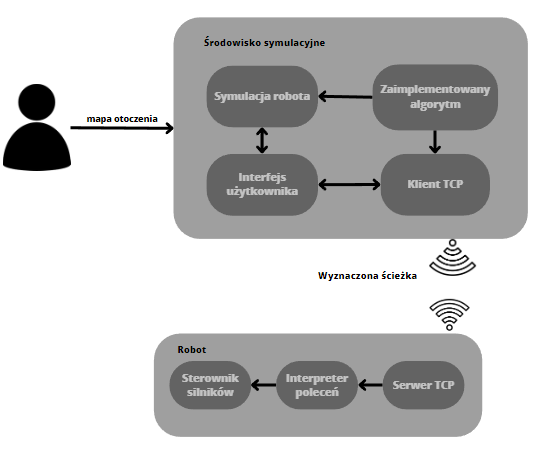
\includegraphics[width=14cm]{pages/literatura/zdjecia/schematOgolny.png}
	\caption{Ogólny schemat projektu}
	\label{sch:ogolnyRozwiazania}
\end{figure}

Użytkownik po uruchomieniu środowiska symulacyjnego będzie miał możliwość edycji mapy opartej na siatce, określenia punktu początkowego i końcowego.
Kolejnym krokiem jest wyznaczenie ścieżki oraz jej graficznej reprezentacji. Tak wyznaczoną ścieżkę można wysłać do robota 
operującego w środowisku rzeczywistym. 
